\scanpage{5}

\diagram{\begin{tikzcd}[ampersand replacement=\&,column sep=1.4em]
{\mathbb Z[\unsure{\mathbb F|F}_{\unsure{n-2|n\,2}}]}
 \& {\mathbb Z[\mathbb F_{n-1}]}\arrow[l]
 \& {\mathbb Z[F_n]}\arrow[l,"{t_n-s_n}"]
 \& {\mathbb Z[\mathbb F_{n+1}]}\arrow[l] \& \unsure{\cdot|\text{,}}
\end{tikzcd}}

\[
\begin{aligned}
D_n&\longrightarrow X &\quad&\deleted{D_n}\unsure{.}\\
\bigl\{x&\in F_n && =\\
t_{n-1}{}&
\underset{\substack{\unsure{E_3}\hfill\\0}}{\underbrace{\vphantom{\bigg|}\bigl(t_n\unsure{(f)|f)}-s_n(f)\bigr)}}
-s_{n-1}\bigl(t_n(f)-s_n\unsure{(f)|f)}\bigr)&&
\end{aligned}
\]

\[
\begin{array}{cc}
\underset{\smile}{F}_0 & F_1\\[.6em]
F'_0 & \mathbb F'_1\\
\unsure{\prime|1}&
\end{array}
\]
\diagram{\begin{tikzcd}[ampersand replacement=\&,column sep=1.7em,row sep=1.3ex]
\&\& \unsure{s}\&\unsure{t}\arrow[l]\\
{\substack{\exists\,\deleted{\unsure{u}}s,u'\\s'}} \&
 f(s)\arrow[l] \& f_0(s) \& f_0(t)\arrow[l]
\end{tikzcd}}

\begin{flushright}
\begin{minipage}{.74\linewidth}
\(\bigl(C_i\bigr)\quad\forall w'\in F'_i,\)
\deleted{if one \unsure{retains|removes|chooses}} \(\deleted{\unsure{s}}\exists w\in\mathbb F_i\) such that
\(f(w)\sim w'\). Moreover if \(i\geq1\), One can
\par\noindent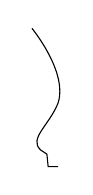
\begin{tikzpicture}[baseline=-2.3em,x=.45em,y=.5em,line width=.4pt]
\draw (0,5)..controls(1.7,3)and(2.6,1)..(2.1,-.4)
 ..controls(1.4,-2)and(-.3,-3)..(.7,-3.8)--(1.2,-4.1)--(1.3,-5)--(2.1,-5);
\end{tikzpicture}\begin{minipage}{.89\linewidth}
\unsure{give} oneself
in advance \(u_{i\unsure{-1}}=s_i(w)\), \inserted{\(v_{i\unsure{-1}}=\)}\(t_i(w)\),
\inserted{\unsure{of|in} \(F_{i-1}\),} subject to the sole conditions \deleted{\unsure{of}} that
\(f(u_{\unsure{i|1}})=u'_{\unsure{i|1}}\), \inserted{\(\unsure{\text{resp}}\)}
\(\unsure{g|f}(v_{\unsure{i|1}})=v'_{\unsure{i|1}}\)
and, \deleted{in} addition, if \(i-1\geq1\) i.e \(i\geq2\), \deleted{\unsure{that}}
\(s(u)=s(v),\ t(u)=t(v)\)
\end{minipage}

(\unsure{NB} one does not require that \(\unsure{g|f}(u)=u'\))
\end{minipage}
\end{flushright}

\[
\begin{aligned}
\unsure{E|\Xi}_0\quad\text{\textcircled{\(\unsure{\mathrm a)|\mathrm b)}\)}}\quad&
\forall s'\in F'_0,\quad \exists s\in F_0,\ u\in F'_1,\quad
f_0(s)\xrightarrow{u}s'\\[-.1em]
&\hspace{4em}\deleted{\pi_0(f)\ \unsure{\text{surj}}}\quad
\unsure{-}\pi_0(f)\ \text{\uuline{\unsure{surj}}}\\
\mathrm b)\quad&
\forall s,t\in F_0,\quad
\underset{\substack{\rotatebox{90}{\(\in\)}\\F'_1}}{u'}:f_0(s)\longrightarrow f_0(t),\\
&\exists u\in\mathbb F_1,\quad u:s\mathbin{-}t\qquad\pi_0(f)\ \text{inj.}
\end{aligned}
\]

\[
\begin{aligned}
E_1\quad\text{\textcircled{\(\mathrm b')\)}}\quad&
\forall s,t\in F_0,\quad
\underset{\substack{\rotatebox{90}{\(\in\)}\\F'_1}}{u'}:
 f_0(s)\mathbin{-} f_0(t),\\
&\exists u\in F_1,\quad u:s\mathbin{-}t,\quad
 f(u)\xrightarrow[\sim]{\unsure{\epsilon|\ell}}u'\\
&\deleted{\unsure{\exists\,w\in F_2}}\\
&\pi_0(f)\ \text{inj. and }\text{\uuline{\(\pi_1(f)\) surj}}
\end{aligned}
\]

\[
\begin{aligned}
\mathrm c)\quad&
\deleted{\forall s,t\in\unsure{\mathbb F_0},}\ u,v\in F_1\quad
\begin{gathered}s_{\unsure{i|1}}(u)=s_1(v),\\[-.2em] t_1(u)=t_1(v)\end{gathered},\\
&\text{and }\underset{\substack{\rotatebox{90}{\(\in\)}\\F'_2}}{w'}:
 f(u)\longrightarrow f(v),\quad
 \exists\underset{\substack{\rotatebox{90}{\(\in\)}\\F_2}}{w}:
 \deleted{\unsure{f|f_1}}u\mathbin{-}v\\
&\pi_{\unsure{1|f}}(f)\ \text{inj.}
\end{aligned}
\]
\diagram{\begin{tikzcd}[ampersand replacement=\&,column sep=2.4em,cells={nodes={inner sep=0pt}}]
{}\arrow[r,bend left=45,"u"]\arrow[r,bend right=45,"v"']\&{}
\end{tikzcd}}

\[
\begin{aligned}
E_2\quad\text{\textcircled{\(\mathrm c'\)}}\quad&
\forall(u,v)\in F_1,\quad
\begin{gathered}s_1(u)=s_1(v)\\[-.2em] t_1(u)=t_1(v)\end{gathered}
\quad\text{and }\underset{\substack{\rotatebox{90}{\(\in\)}\\F'_2}}{w'}:
 f(u)\mathbin{-}f(v),\\
&\exists\underset{\substack{\rotatebox{90}{\(\in\)}\\F_2}}{w}:u\longrightarrow v\
 \deleted{\unsure{and|f}}\ \text{such that}\\
&w'\sim f(w)\qquad\overbrace{\pi_1(f)\ \text{inj and }\pi_2(f)\ \text{surj}}
\end{aligned}
\]
\diagram{\begin{tikzcd}[ampersand replacement=\&,column sep=1.7em,cells={nodes={inner sep=0pt}}]
{}\arrow[r,bend left=46,dash,"{f(u)}"]\arrow[r,bend right=42,dash]
 \arrow[r,draw=none,"{w'\!\downarrow}" description]\&{}
\end{tikzcd}}
% archive sheet number: 4
